\begin{frame}
  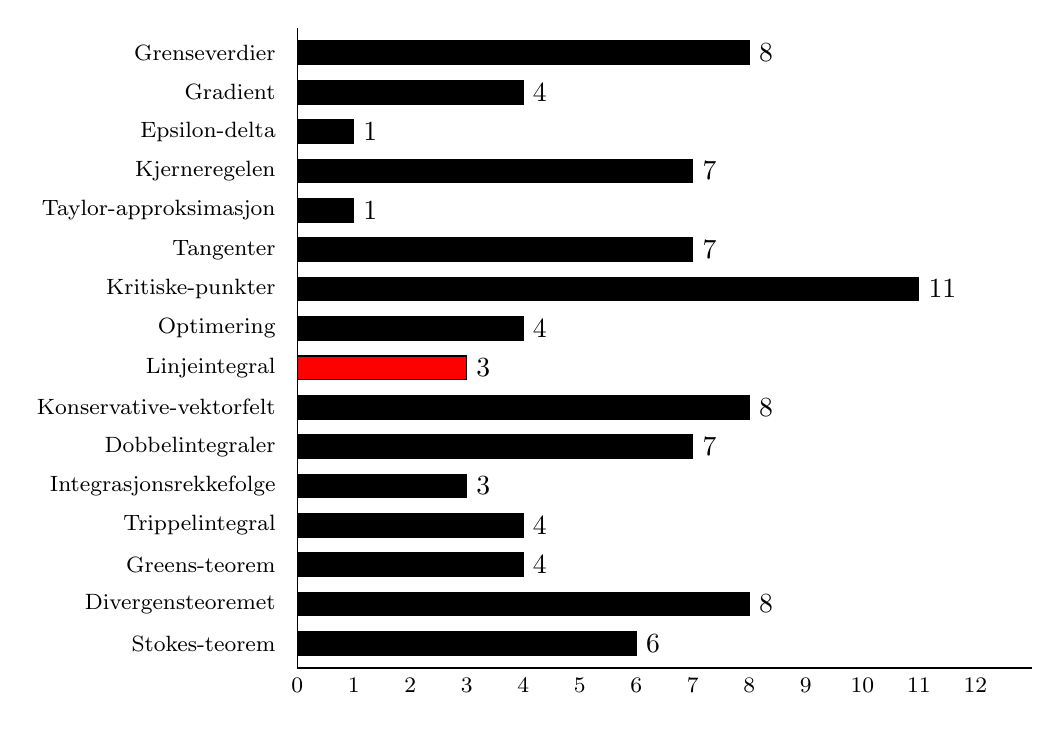
\begin{tikzpicture}
    \begin{axis}[ xbar=0pt, /pgf/bar shift=0pt, legend style={ legend columns=4,
        at={(xticklabel cs:0.5)}, anchor=north, draw=none }, ytick={0,...,15},
      ytick style={draw=none},% <- added
      axis y line*=none, axis x line*=bottom, tick label
      style={font=\footnotesize}, legend style={font=\footnotesize}, label
      style={font=\footnotesize}, xtick style={draw=none},% <- added
      xtick={0,1,...,12}, width=.9\textwidth, bar width=3mm, y dir = reverse,
      xmin=0, xmax=13, area legend,
      y=5mm, enlarge y limits={abs=0.625},
      style={text=black}, every axis plot/.append style={fill},
      nodes near coords, nodes near coords,
      yticklabels={%
        {\topicref{Grenseverdier}},
        {\topicref{Gradient}},
        {\topicref{Epsilon-delta}},
        {\topicref{Kjerneregelen}},
        {\topicref{Taylor-approksimasjon}},
        {\topicref{Tangenter}},
        {\topicref{Kritiske-punkter}},
        {\topicref{Optimering}},
        {\topicref{Linjeintegral}},
        {\topicref{Konservative-vektorfelt}},
        {\topicref{Dobbelintegraler}},
        {\topicref{Integrasjonsrekkefolge}},
        {\topicref{Trippelintegral}},
        {\topicref{Greens-teorem}},
        {\topicref{Divergensteoremet}},
        {\topicref{Stokes-teorem}}}]
      \addplot[fill=black] coordinates {(8,0)};
      \addplot[fill=black] coordinates {(4,1)};
      \addplot[fill=black] coordinates {(1,2)};
      \addplot[fill=black] coordinates {(7,3)};
      \addplot[fill=black] coordinates {(1,4)};
      \addplot[fill=black] coordinates {(7,5)};
      \addplot[fill=black] coordinates {(11,6)};
      \addplot[fill=black] coordinates {(4,7)};
      \addplot[fill=red] coordinates {(3,8)};
      \addplot[fill=black] coordinates {(8,9)};
      \addplot[fill=black] coordinates {(7,10)};
      \addplot[fill=black] coordinates {(3,11)};
      \addplot[fill=black] coordinates {(4,12)};
      \addplot[fill=black] coordinates {(4,13)};
      \addplot[fill=black] coordinates {(8,14)};
      \addplot[fill=black] coordinates {(6,15)};
    \end{axis}
  \end{tikzpicture}
\end{frame}

\begin{frame}
  \subsection{Linjeintegral}\label{subsec:Linjeintegral}
  \frametitle{Linjeintegral}
  \centerline{%
    \only<1>{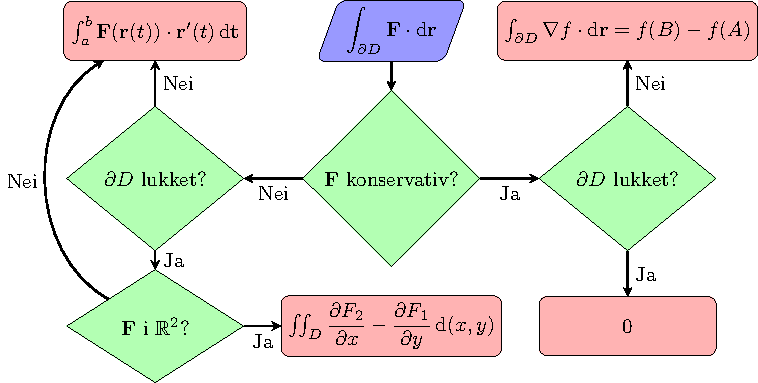
\includegraphics[scale=0.95]{../img/flytskjema-linjeintegral}}%
    \only<2>{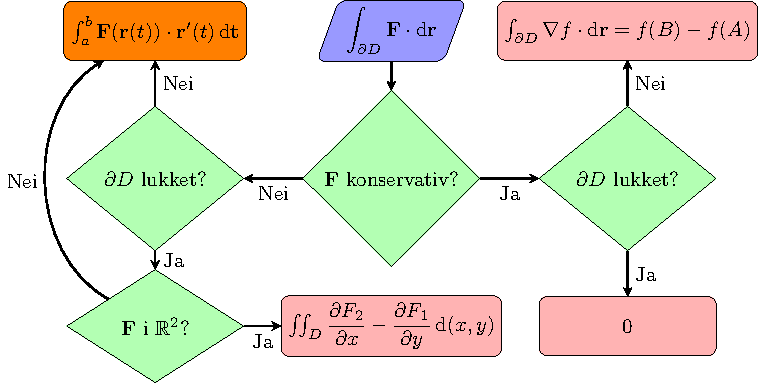
\includegraphics[scale=0.95]{../img/flytskjema-linjeintegral-1}}
  }
  $\partial D$ er en kurve slik at $\partial D \colon \rr(t), \ a \leq t \leq b$
  med $\rr(a)=A$ og $\rr(b) = B$. \\
  $D$ er området avgrenset av $\partial D$. Dersom $\F$ er konservativ er $\nabla f = \F$.
\end{frame}

\begin{frame}
  \begin{columns}
    \column{0.58\linewidth}
  \begin{oppgave}{K2016, Oppgave 6}
    La $\F(x,y) = (0, x)$. Hva er verdien av integralet
    %
    \begin{equation*}
      \int_C \F \cdot \dr
    \end{equation*}
    %
    der $C$ er en sirkel med radius $a > 0$? 
  \end{oppgave}
  
  \column{0.38\linewidth} \vspace{0.5cm}
  \only<1>{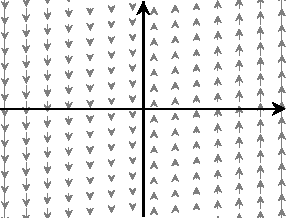
\includegraphics{../img/vektorfelt-linjeintegral-0}}
  \only<2>{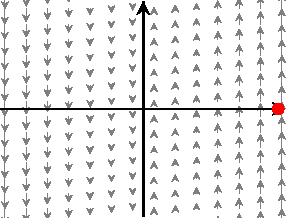
\includegraphics{../img/vektorfelt-linjeintegral-1}}
  \only<3>{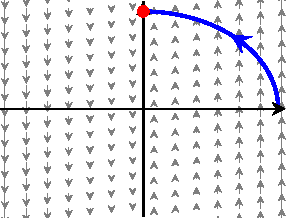
\includegraphics{../img/vektorfelt-linjeintegral-2}}
  \only<4>{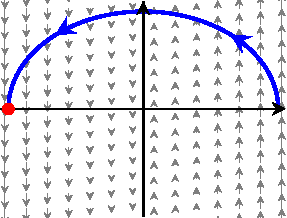
\includegraphics{../img/vektorfelt-linjeintegral-3}}
  \only<5>{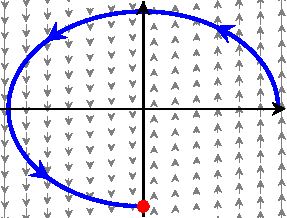
\includegraphics{../img/vektorfelt-linjeintegral-4}}
  \only<6->{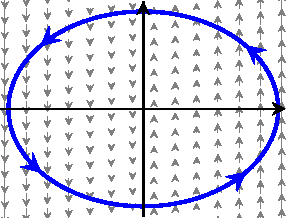
\includegraphics{../img/vektorfelt-linjeintegral}}
  \end{columns}
    \begin{align*}
    \rr\phantom{'}(\theta)
    & = (x_0 + a \cos \only<1>{\theta}\only<2>{0}\only<3>{\frac{\pi}{2}}\only<4>{\pi}\only<5>{\frac{3\pi}{2}}\only<6->{\theta}) \I
      + (y_0 + a \sin \only<1>{\theta}\only<2>{0}\only<3>{\frac{\pi}{2}}\only<4>{\pi}\only<5>{\frac{3\pi}{2}}\only<6->{\theta}) \J \hfill \visible<8->{\\
  \rr'(\theta) & = \hspace{0.75cm} - a \sin \theta\phantom{)}\I + \hspace{0.8cm} (a \cos \theta) \J\\
    \F\bigl(\rr(\theta)\bigr) & = \hspace{1.85cm} 0 \phantom{)} \I + \hspace{-0.05cm} (x_0 + a \cos \theta) \J \\}
    \visible<7->{
    \int_C \F \cdot \dr
    & = \int_0^{2\pi} \F\bigl( \rr(\theta) \bigr) \rr'(\theta) \dT \\} \visible<9->{
      & = \int_0^{2\pi} ax_0 (\cos \theta) + a^2 (\cos \theta)^2 \dT } \visible<10->{
      = \int_0^{2\pi} \frac{a^2}{2} \dT 
      =  \pi a^2 }
    \end{align*}
  \end{frame}

  \begin{frame}
\frametitle{Trigonometri: like funksjoner}
    \begin{tikzpicture}
        \begin{axis}[
            Trigonometric Style,
            legend style={at={(0.68,1)},anchor=north east},
            legend style = {draw = none},
            legend style = {fill=none},
            xtick={
                -6.28318, -4.7123889, -3.14159, -1.5708,
                1.5708, 3.14159, 4.7123889, 6.28318
            },
            xticklabels={
                $-2\pi$, $-\frac{3\pi}{2}$, $-\pi$, $-\frac{\pi}{2}$,
                $\frac{\pi}{2}$, $\pi$, $\frac{3\pi}{2}$, $2\pi$
            }
        ]
        \addplot [mark=none, ultra thick, red] {cos(deg(x))^2};
        \addplot [mark=none, ultra thick, blue] {sin(deg(x))^2};
        \legend{$(\cos x)^2$,$(\sin x)^2$}
        \end{axis}
    \end{tikzpicture}
    \begin{theorem}
    Det å integrere $(\cos x)^2$ eller $(\sin x)^2$ over intervaler som er multiplum av $\pi/2$ er det samme som å integrere $1/2$ over samme intervalet:
        \begin{align*}
              \int_{m\pi/2}^{n\pi/2} (\sin x)^2 \mathrm{d}x
            = \int_{m\pi/2}^{n\pi/2}  (\cos x)^2 \mathrm{d}x
            = \frac{1}{2} \int_{m\pi/2}^{n\pi/2}  \mathrm{d}x \qquad m,n \in \mathbb{Z}
    \end{align*}
    \end{theorem}
  \end{frame}

  \begin{frame}
    \begin{tikzpicture}
        \begin{axis}[
            Trigonometric Style,
            legend style={at={(0.68,1)},anchor=north east},
            legend style = {draw = none},
            legend style = {fill=none},
            xtick={
                -6.28318, -4.7123889, -3.14159, -1.5708,
                1.5708, 3.14159, 4.7123889, 6.28318
            },
            xticklabels={
                $-2\pi$, $-\frac{3\pi}{2}$, $-\pi$, $-\frac{\pi}{2}$,
                $\frac{\pi}{2}$, $\pi$, $\frac{3\pi}{2}$, $2\pi$
            }
        ]
        \addplot [mark=none, ultra thick, red] {cos(deg(x))^2};
        \addplot [mark=none, ultra thick, blue] {sin(deg(x))^2};
        \legend{$(\cos x)^2$,$(\sin x)^2$}
        \end{axis}
      \end{tikzpicture}
      \begin{align}
        &\int_0^{\pi/2} (\sin x)^2 \dx
        \only<1>{ \overset{u \mapsto x - \pi/2}{=} -\int_{\pi/2}^0 (\sin(\pi/2 - u))^2 \du}
        \only<2->{= \int_0^{\pi/2} (\cos x)^2 \dx }
        \only<3>{\\ & (\cos x)^2 + (\sin x)^2 = 1}\only<4>{\\ & \int_0^{\pi/2} (\sin x)^2 + (\cos x)^2 \dx = \int_0^{\pi/2} 1 \dx}\only<5->{\\ & \int_0^{\pi/2} (\sin x)^2\dx + \int_0^{\pi/2}(\cos x)^2 \dx = \int_0^{\pi/2} 1 \dx}
                                                                                                                          \visible<6->{\\  & \hspace{3cm}\Downarrow \notag \\
        &\int_0^{\pi/2} (\sin x)^2 \dx = \int_0^{\pi/2} (\cos x)^2 \dx  = \int_0^{\pi/2} \frac{\dx}{2}}
      \end{align}
  \end{frame}

%%% Local Variables:
%%% mode: latex
%%% TeX-master: "main"
%%% End:
